
\documentclass[a4paper]{article}

\usepackage{inputenc}
\usepackage[british,UKenglish]{babel}
\usepackage{amsmath}
%\usepackage{titlesec}
\usepackage{color}
\usepackage{graphicx}
\usepackage{fancyref}
\usepackage{hyperref}
\usepackage{float}
\usepackage{scrextend}
\usepackage{setspace}
\usepackage{xargs}
\usepackage{multicol}
\usepackage{nameref}

\usepackage{sectsty}
\usepackage{multicol}
\usepackage{multirow}
\usepackage[procnames]{listings}
\usepackage{appendix}
\usepackage{listings}
\usepackage{booktabs} % 导入三线表需要的宏包
\usepackage{array}
\usepackage{indentfirst} 
\setlength{\parindent}{2em} %段落缩进

\newcommand\tab[1][1cm]{\hspace*{#1}}
\hypersetup{colorlinks=true, linkcolor=black}
\interfootnotelinepenalty=10000

\newcommand{\cleancode}[1]{\begin{addmargin}[3em]{3em}\texttt{\textcolor{cleanOrange}{#1}}\end{addmargin}}
\newcommand{\cleanstyle}[1]{\text{\textcolor{cleanOrange}{\texttt{#1}}}}


\usepackage[colorinlistoftodos,prependcaption,textsize=footnotesize]{todonotes}
\newcommandx{\commred}[2][1=]{\textcolor{Red}
{\todo[linecolor=red,backgroundcolor=red!25,bordercolor=red,#1]{#2}}}
\newcommandx{\commblue}[2][1=]{\textcolor{Blue}
{\todo[linecolor=blue,backgroundcolor=blue!25,bordercolor=blue,#1]{#2}}}
\newcommandx{\commgreen}[2][1=]{\textcolor{OliveGreen}{\todo[linecolor=OliveGreen,backgroundcolor=OliveGreen!25,bordercolor=OliveGreen,#1]{#2}}}
\newcommandx{\commpurp}[2][1=]{\textcolor{Plum}{\todo[linecolor=Plum,backgroundcolor=Plum!25,bordercolor=Plum,#1]{#2}}}

\def\code#1{{\tt #1}}

\def\note#1{\noindent{\bf [Note: #1]}}

\makeatletter
%% The "\@seccntformat" command is an auxiliary command
%% (see pp. 26f. of 'The LaTeX Companion,' 2nd. ed.)
\def\@seccntformat#1{\@ifundefined{#1@cntformat}%
   {\csname the#1\endcsname\quad}  % default
   {\csname #1@cntformat\endcsname}% enable individual control
}
\let\oldappendix\appendix %% save current definition of \appendix
\renewcommand\appendix{%
    \oldappendix
    \newcommand{\section@cntformat}{\appendixname~\thesection\quad}
}
\makeatother




\lstset{frame=, basicstyle={\footnotesize\ttfamily}}



\graphicspath{ {images/} }
\usepackage{ctex}



\usepackage[square,numbers]{natbib}
\bibliographystyle{abbrvnat}


\begin{document}
\renewcommand{\contentsname}{目\ 录}
\renewcommand{\appendixname}{附录}
\renewcommand{\appendixpagename}{附录}
\renewcommand{\refname}{参考文献}

\renewcommand{\tablename}{表}
\renewcommand{\today}{\number\year 年 \number\month 月 \number\day 日}

\title{{\Huge 可视语言与信息可视化{\large\linebreak\\}}{\Large 团队ID: \linebreak}
{\Large  \linebreak\linebreak}}
\author{ \large
  刘京宗 3019213043
  \\\\
  杨朝涵 3020244160
  \\\\
  张雪雅 3020244317
  \\\\\\
  天津大学,智能与计算学部}
\date{\today}
\maketitle
\newpage

\begin{center}
  \tableofcontents\label{c}
\end{center}
\newpage


\begin{center}
  {\Large\bf{摘\ 要\\}}

  大作业要求大家按照论文短文的格式进行书写,参考文献~\cite{bayrak2020pragma, govyadinov2019graph}。



\end{center}

\newpage



\section{引言}
\label{overview}
\begin{figure}[htbp]
  \centering
  
\includegraphics[width=1\textwidth]{images/MC3.jpg}
  \caption{背景}\label{fig:MC3}
  \vspace{\baselineskip}
\end{figure}
2014年1月23日,阿比拉发生了多起事件。系统已要求您根据发生的有限信息进行回顾性分析。您的目标是确定风险以及如何更有效地缓解风险。

您可以访问包含两个主要来源的单个数据流:

由自动筛选器识别为与正在进行的事件潜在相关的微博记录

阿比拉,克罗诺斯岛地方警察和消防部门的紧急调度文字记录。

根据这些数据,您可以评估公众不断变化的风险水平并提出建议的措施吗?

您还可以访问阿比拉地图和背景文件。 (注意:这些是“迷你挑战1”和“迷你挑战2”中提供的相同材料)

使用视觉分析来分析可用数据并制定对要提供的问题的响应。此外,准备一段视频,展示您如何使用视觉分析来解决这一难题。

\section{相关工作}

调研相关论文发表,搜索CNKI或者Google scholar 等学术引擎,了解该领域研究现状。参考文献格式为~\cite{bayrak2020pragma}。

\section{问题描述和需求分析}
\label{Data and Task Abstraction}
使用视觉分析来表征数据集中不同类型的内容。什么是有意义的事件报告与典型的垃圾邮件或垃圾邮件区别开来?请将答案限制为8张图片和500个单词。

使用可视化分析来表示和评估在晚上的过程中对公众的风险程度如何演变。考虑这种情况的潜在后果以及可能受到影响的人数。请将答案限制为10张图片和1000字。

如果您能够将一组急救人员发送到任何地方,它将在哪里?提供您的理由。如果您必须实时而不是回顾性地响应事件,那么您的响应会有什么不同?请将答案限制为8张图片和500个单词。

\section{解决方案}
\subsection*{ 4.1 任务一}
(1)借助Python处理数据,提取message中的tag,并且统计每个tag出现的次数,据此绘制词云。

(2)借助Python处理数据,对message进行分类,借助散点图和柱状图表征数据集中不同类型的内容。

(3)使用tf-idf算法,对不同类型的message提取关键词,并且用TreeMap展示。

(4)统计不同类型的message的作者信息,同样用TreeMap进行展示。
\subsection*{ 4.2 任务二}
\subsection*{ 4.3 任务三}

\section{实验结果和案例分析}\label{sub:ptxeva}
\subsection*{ 5.1 任务一}

统计不同tag在message中出现的次数,如图~\ref{fig:1-tags}~所示。

\begin{figure}[H]
  \centering
  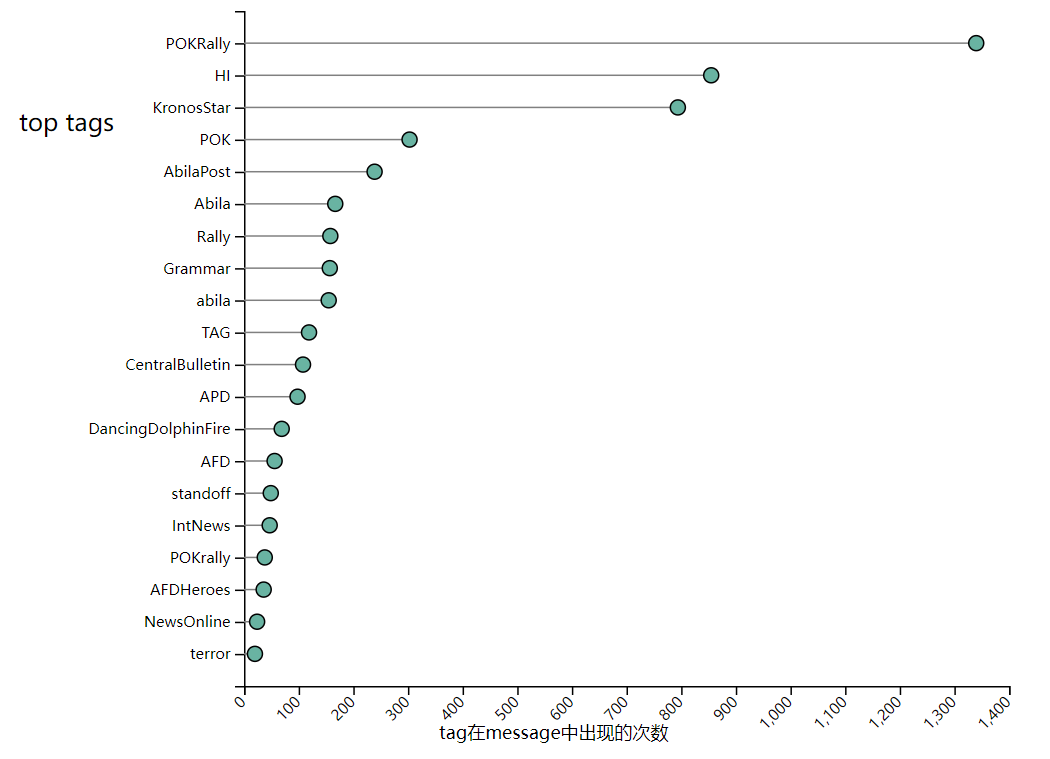
\includegraphics[width=0.9\textwidth]{images/1-tags.png}
  \caption{不同tag在message中出现的次数}\label{fig:1-tags}
  \vspace{\baselineskip}
\end{figure}
\begin{figure}[H]
  \centering
  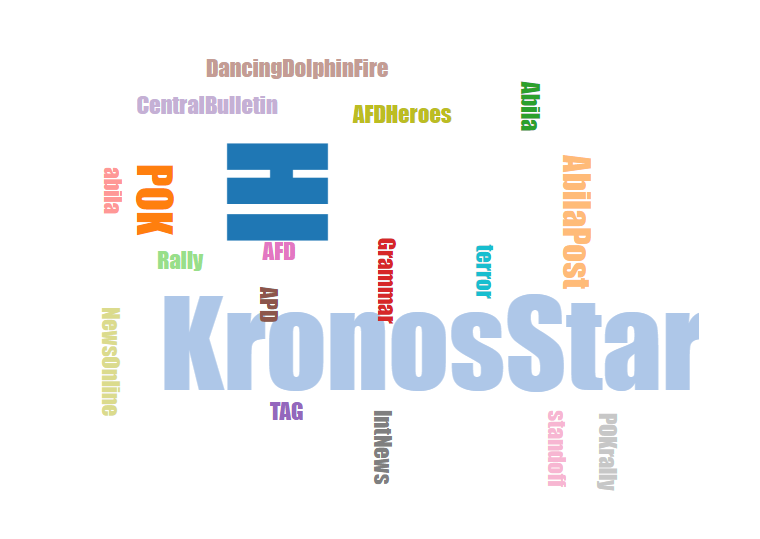
\includegraphics[width=0.8\textwidth]{images/1-wordcloud.png}
  \caption{tag词云}\label{fig:1-wordcloud}
  \vspace{\baselineskip}
\end{figure}
通过这些tag,我们可以对message的主题有一个把握,并且词云的形象化展示,让我们对数据有了更直观的认识。

借助Python处理数据,对message进行分类,具体如表~\ref{tab:table1}~所示。
\begin{table}[H]
  \caption{不同类别的message分类说明}\label{tab:table1}
  \vspace{0.5em}\centering
  %设置表格的宽度不超过页面长度
  \begin{tabular}{|p{2.2cm}<{\raggedright}|p{8.5cm}<{\raggedright}|}
    \toprule[1.5pt]
    种类          & 说明                                                                                                                                      \\                                                                                                                               \\
    \midrule[1pt]
    unrelated     & 与报道完全无关的消息。主要由用户@KronosQuoth和@Clevvah4Evah发出。二人的消息主要是一些“心灵鸡汤”、励志格言,与报道内容完全无关,共1418条。 \\ \hline
    advertisement & 广告。其内容中往往包含了网页链接,如“I recommend this site \#abila dates.kronos/clickhere” 借助正则表达式'.*\..*/'进行筛选,共227条。      \\ \hline
    chatter       & 闲聊。这部分内容主要为用户的闲聊,主要特征为通常以“RT @”开头,共1006条                                                                    \\ \hline
    report        & 报道。主要为当地媒体对新闻的报导,如关于火灾,枪击的报道。主要由@AbilaPost, @megaMan等用户发送,共424条。                                 \\ \hline
    others        & 其他。不能被以上四类所典型概括的消息,统一归为其他,共988条。                                                                             \\ \hline
    \bottomrule[1.5pt]
  \end{tabular}
  \vspace{\baselineskip}
\end{table}
在对message进行分类后,我们采用散点图和柱状图表征数据集中不同类型message的内容.
\begin{figure}[H]
  \centering
  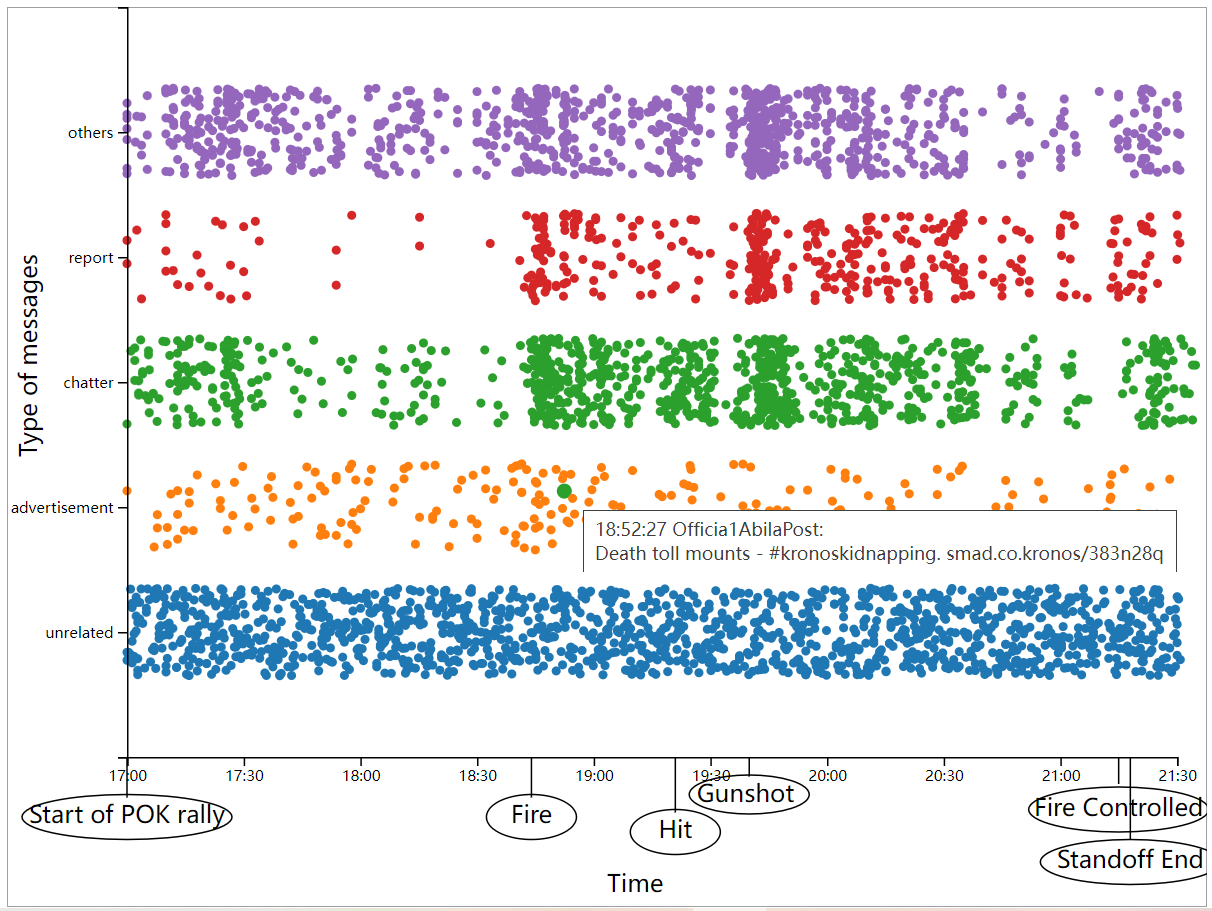
\includegraphics[width=0.95\textwidth]{images/1-scatter-2.png}
  \caption{散点图}\label{fig:1-scatter}
  \vspace{\baselineskip}
\end{figure}
\begin{figure}[H]
  \centering
  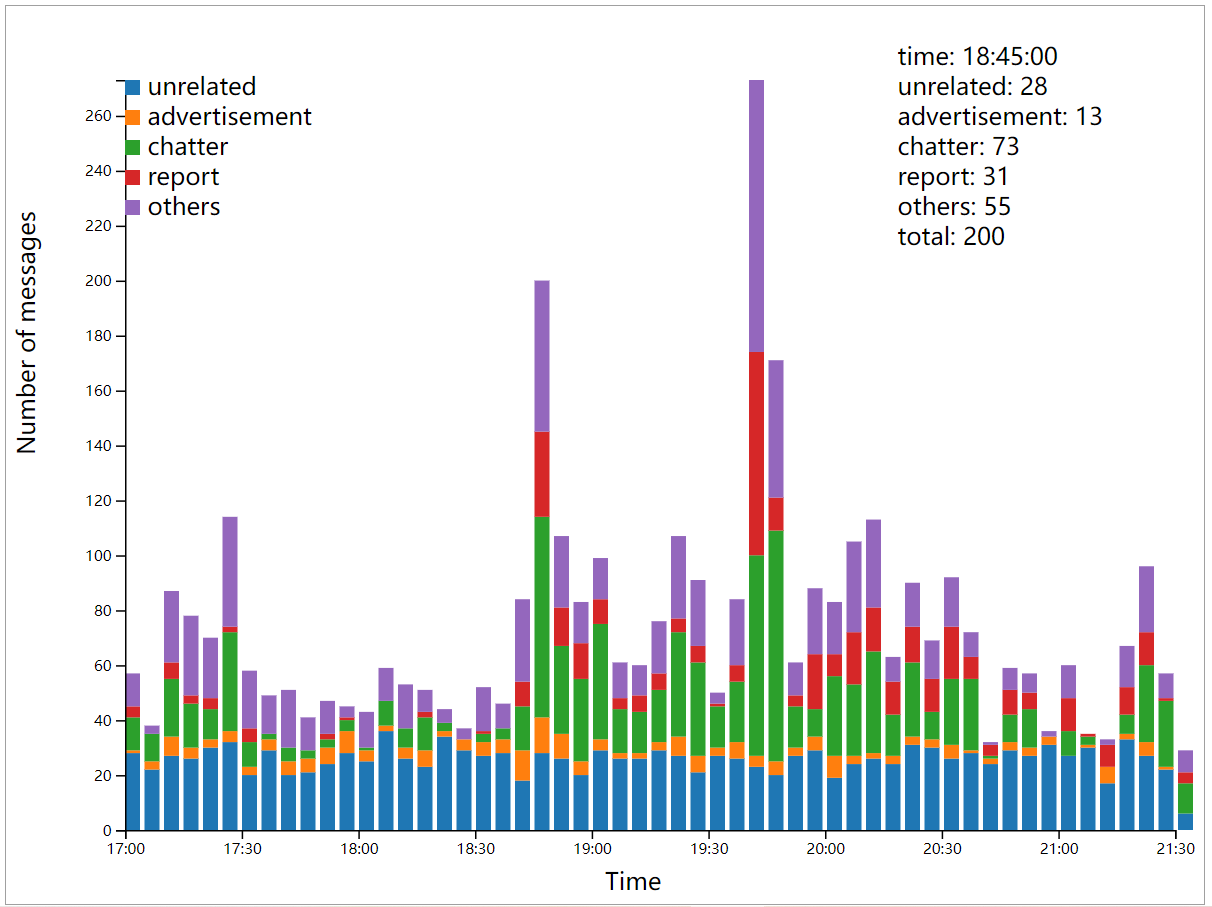
\includegraphics[width=1\textwidth]{images/1-bars-2.png}
  \caption{柱状图}\label{fig:1-bar}
  \vspace{\baselineskip}
\end{figure}
通过散点图和柱状图,我们可以对不同类型的message随时间的变化有一个直观的认识。且我们能直观感受到有重大事件(如图~\ref{fig:1-scatter}~横轴所示)发生时,
chatter和report类型的消息数量会有一个明显增加。
且我们为这两幅图增加了一定的交互性,当鼠标悬停在散点图中的点上时,会
有颜色变化,同时显示出该点对应的message信息,包括时间与作者信息。当
鼠标悬停在柱状图中的柱子上时,会显示出该柱子对应的时间段以及该时间段内
的各种message的数量。



\subsection*{ 5.2 任务二}
\subsection*{ 5.3 任务三}
\section{总结}

\bibliography{ref}

\end{document}

